\section{Simulation Experiments} \label{sec:exp}

\begin{table}[tbh]
    \centering
\begin{small}
\begin{tabular}{lrrrr}
\toprule
& \multicolumn{2}{c}{Test Accuracy } & RMS & Max \\
Mechanism &  $\epsilon = 2$ &  $\epsilon = 8$ & Loss & Loss\\

%%%%%%%%%%%%%%%%%%%%%%%%%%%%%
% Left columns
% AUTO-GENERATED, loss added manually, see
%https://colab.corp.google.com/drive/1vaZjMTrTIPDmTTsRtc-Rm7l_LEJUqKe6#scrollTo=QzeNkbKQWHxN&uniqifier=2
\midrule
\bandmf(band=342)\ifthenelse{\boolean{acl}}{}{~\citep{choquette2023amplified}} & 23.21 & 24.86 & 10.21 & 8.60 \\
\tafull\ifthenelse{\boolean{acl}}{}{~\citep{denisov22matfact}} & 22.54 & 24.47 & 14.98 & 12.47 \\
\blt(nbuf=2,$k$=1)\ifthenelse{\boolean{acl}}{}{~\citep{mcmahan2024efficient}} & 22.37 & 24.64 & 11.80 & 11.15 \\
\blt(nbuf=5,$k$=1)\ifthenelse{\boolean{acl}}{}{~\citep{mcmahan2024efficient}} & 22.40 & 24.63 & 11.40 & 10.87 \\
\blt*(nbuf=2,$k$=6) & 23.09 & 24.83 & 10.81 & 9.34 \\
\blt*(nbuf=3,$k$=6) & 23.13 & 24.87 & 10.79 & 9.33 \\
\blt*(nbuf=4,$k$=6) & 23.13 & 24.83 & 10.79 & 9.33 \\
\blt*(nbuf=5,$k$=6) & 23.07 & 24.84 & 10.79 & 9.33 \\
\bottomrule
\end{tabular}
\end{small}
% End AUTO-GENERATED
%%%%%%%%%%%%%%%%%%%%%%%%%%%%%
    \caption{\small Comparing mechanisms in terms of test-set accuracy on the StackOverflow NWP task. All runs are based on $\nd=2052$ rounds of training with $\maxpart=6$ participations and min-sep $\minsep=342$. \blts are optimized for \maxloss. Results are visualized in \cref{fig:sonwp} in \cref{app:plots}.}
    \label{tab:sonwp}
    \vspace{-0.4cm}
\end{table}

We run simulation experiments before applying our BLT-DP-FTRL algorithm in \cref{sec:background_blt} to train production LMs. The BLT parameters $(\theta, \omega)$ are optimized with our multi-participation approach in \cref{sec:blt_mp}. We present private-utility trade-off on StackOverflow benchmark dataset in \cref{sec:sonwp}, and \maxloss, \rmsloss across a range of scenarios in \cref{sec:rmse_exp}. We compare \blts to both flexible \treeagg~\citep{kairouz21practical} and state-of-the-art \bandmf~\citep{choquette2023amplified} (see \cref{sec:background} for more discussion). 
In the simulation experiments, we are \emph{maximally generous} in evaluating \treeagg mechanisms, considering the memory cost to be $\ceil{\log_2 \nd}$, while calculating \rmse and \maxerr using the optimal \tafull~\citep{denisov22matfact} without memory-efficient implementation, and use the lower bound of \cref{rem:senslb} to account for overly optimistic privacy-utility trade-off. Thus, in all cases we over-estimates the true performance of the binary tree, but nevertheless we show \blts have superior performance in terms of both error and memory.

% \subsection{Baselines}\label{sec:baselines}
% We consider the following mechanism
% \begin{itemize}
%     \item \blt mechanisms, introduced for single participation by \citet{mcmahan2024efficient}, and using techniques introduced here, optimized for \bparticipation under \rmse and \maxerr. \bnote{TODO - think about whether we need to do this.}
 
%     \item \bandmf \citep{choquette2023amplified}, which optimizes arbitrary (e.g., not Toeplitz) banded $\bfC$ for \bparticipation under \rmse. 

%     \item \bandtoep \citep{mckenna2024scaling}, which optimizes banded Toeplitz matrices $\bfC$ for \bparticipation under \rmse. The primary advantage of this mechanism compared to \bandmf is that \bandtoep matrices can be optimized for much larger $\nd$.
    
%     \item Several schemes based on binary \treeagg for prefix sums appear in the literature.  Prior work on DP-FTRL \citep{kairouz21practical} used the streaming (``from below'') estimator of  \citet{honaker15efficient}, but \citet{denisov22matfact} showed that in fact the ``fully efficient''\footnote{Here ``fully efficient'' referes to the statistical efficiency of the estimator of the prefix sum, not the memory or time efficiency of noise generation} estimator of \citet{honaker15efficient} (the Moore-Penrose pseudoinverse of the binary tree matrix $\bfC$) could in fact be used in the streaming setting. A memory-efficient implementation of streaming ``fully efficient'' estimation is not known, and other works (e.g. \citet{andersson24smooth}) consider alternative memory-efficient approaches. Hence, for simplicity, we are \emph{maximally generous} in evaluating \treeagg mechanisms, considering the memory cost to be $\ceil{\log_2 \nd}$ (the minimum for any estimator), while calculating \rmse and \maxerr using the optimal (but possibly not memory efficient) pseudo-inverse estimator. Finally, we use the easy-to-compute sensitivity lower bound of \cref{rem:senslb}, which though apparently tight could under-estimate the sensitivity of \treeagg. Thus, in all cases we over-estimates the true performance of the binary tree, but nevertheless we show \blts have superior performance in terms of both error and memory.

\begin{figure}[htb]
    \centering
    % From https://colab.corp.google.com/drive/1_BRrt0jUniaOixKwasKDr7jiSToRwJLj#scrollTo=bPzQxRSvA3rk&uniqifier=1
    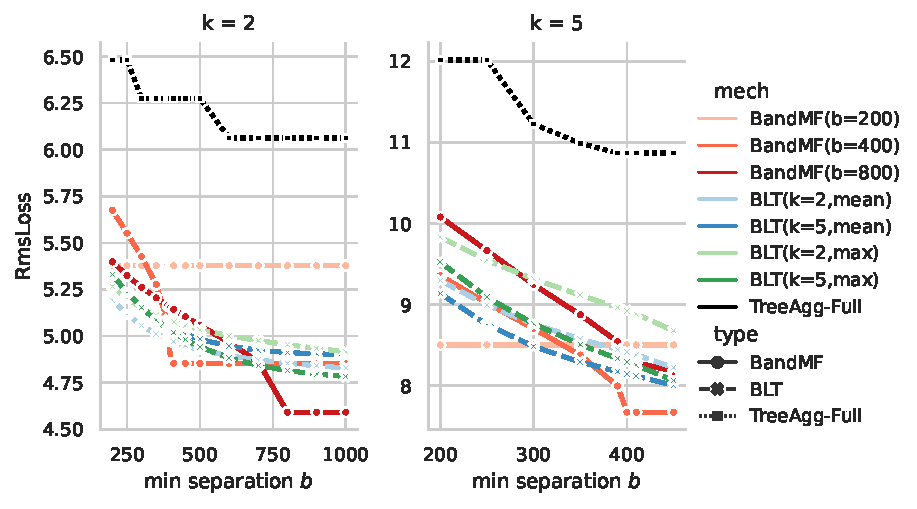
\includegraphics[width=0.9\linewidth]{images/rmsloss_k25.pdf}
    \caption{\small Comparison of mechanisms in terms of prefix-sum root-mean-squared error at a fixed privacy level. \blts were optimized for either \rmsloss (``mean'') or \maxloss (``max''), and for either $\maxpart=2$ or $\maxpart=5$ participations at min-separation $\minsep=400$. BandMF matrices were optimized for $\minsep \in \{200, 400, 800\}$ (the \bandmf optimization does not depend on $\maxpart$, and previous work optimizes for \rmsloss). %Thus $b=400$ lines at $k=2$ and $k=5$ correspond to the scenarios targeted directly by optimization; the other $k$ and min-separation values show how well the mechanisms generalize to other scenarios. 
    We also include \tafull using the optimal (``full Honaker'') decoding (for which a memory-efficient noise generation algorithm is unknown). 
    \textbf{We observe that all the \blts perform competitively with \bandmf, and can outperform \bandmf} when the min-separation differs significantly from the number of bands. For example, with $k=2$ participations (left panel) our BLT($k=2$,mean) (light blue) BLT outperforms BandMF($b=400$) when min separation is less than 390 or greater than 700. 
    }
    \vspace{-0.4cm}
    \label{fig:rmse}
\end{figure}

\subsection{StackOverflow NWP Benchmark} \label{sec:sonwp}

We follow \citet{choquette2023amplified} for StackOverflow next word prediction (NWP) experiments, including all hyperparameter tuning, and vary only the DP mechanism to compare \bandmf, \tafull, and \blts. Results are summarized in \cref{tab:sonwp}. \bandmf still achieves the highest performance, as in this scenario we train for a fixed known number of rounds, with an exactly known max participations $\maxpart=6$ and min-separation $\minsep=342$. \tafull and \blts optimized for only $\maxpart=1$ participation~\citep{mcmahan2024efficient} are noticeably worse, but our multi-participation-optimized \blts are very competitive with \bandmf with only 2 or 3 buffers (with a $171\times$ and $114\times$ reduction in runtime memory overhead). 
\ifthenelse{\boolean{acl}}{}{We expect the negligibly worse performance of larger numbers of buffers may be due to the impact of regularization during the optimization of the \blt parameters.}
In the relatively large signal-to-noise ratio regime ($\epsilon=8$), \ourblt achieves comparable or even better learning accuracy though the \rmsloss (\maxloss) is slightly worse.


\subsection{\rmsloss and \maxloss Experiments} \label{sec:rmse_exp}

\paragraph{Comparing BLT to \tafull and \bandmf} We further show that \blt is better than {\small \tafull}, and more flexible than \bandmf by computing \rmsloss (\maxloss) in a wide range of scenarios. Because the \bandmf mechanisms are optimized for \rmsloss, we compare on this metric in \cref{fig:rmse}. However, in both our StackOverflow and Gboard experiments described subsequently, we deploy BLT mechanisms optimized for \maxerr following \citep{mcmahan2024efficient}. For completeness, we provide \cref{fig:maxloss} in \cref{app:plots} that compares the mechanisms on \maxloss. 
\ifthenelse{\boolean{acl}}{}{The BLTs directly optimized for the metric perform better than optimizing for a different metric.} 
We observe that \emph{all the \blts perform competitively with \bandmf, and can outperform \bandmf} when the min-sep differs significantly from the number of bands. For example, in \cref{fig:rmse}, with $k=2$ participations (left panel) our BLT($k=2$,mean) (light blue) BLT outperforms BandMF($b=400$) when min separation is less than 390 or greater than 700. 

\ifthenelse{\boolean{acl}}{We provide more results on the robustness of \blts to min-sep $b$, number of rounds $n$, and comparing with \bandtoep in \cref{app:mse}.  }{
\begin{figure}[H]
    \centering
    % FROM: TODO
    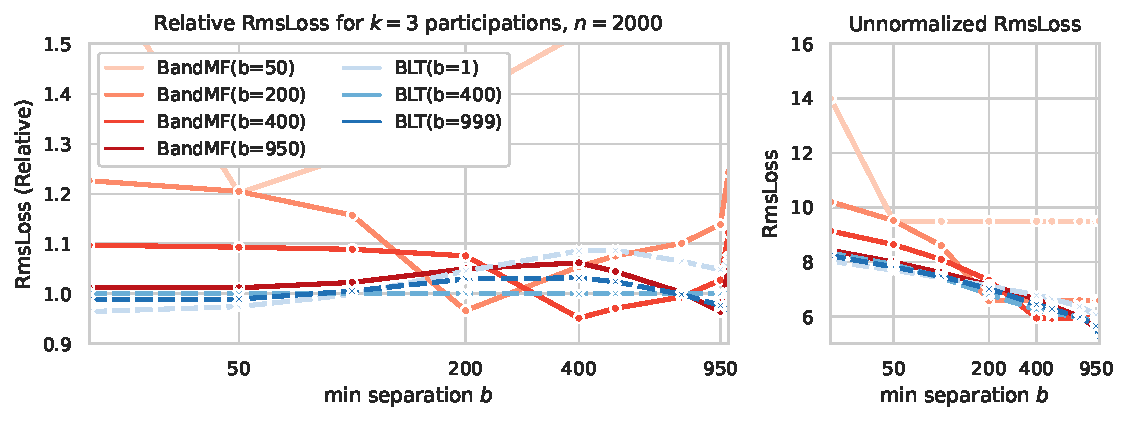
\includegraphics[width=\linewidth]{images/rmse_vary_min_sep_k3.pdf}
    \caption{Comparison of \bandmf and \blts with $\nd = 2000$ and $k=3$ participations, varying the min-separation $\minsep$. The \blts were optimized for \rmsloss. The $x$-axis is shown on a log-scale. The left panel gives loss relative to the $\bltm(b=400)$ mechanism, while the right panel gives the same data on an unnormalized $y$-axis scale.}
    \label{fig:rmse_k3}
\end{figure}

\begin{figure}[H]
    \centering
    % FROM: TODO
    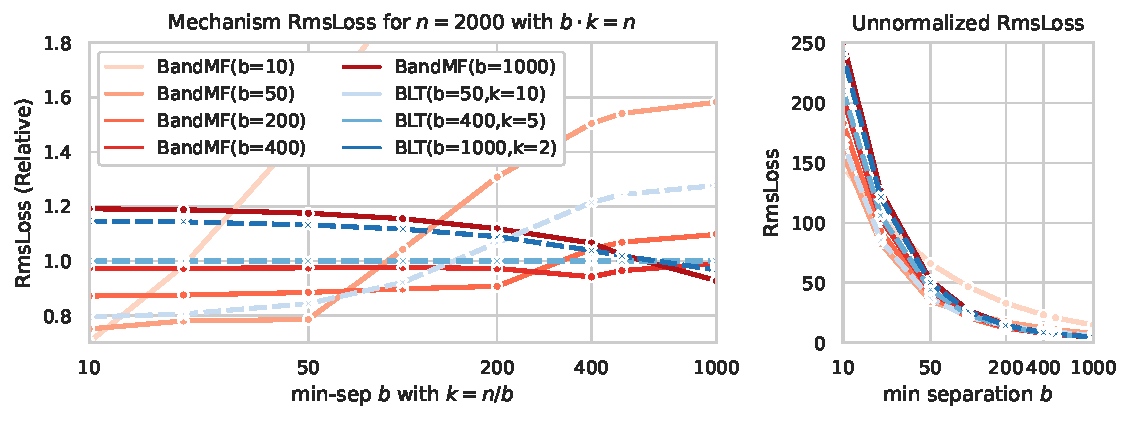
\includegraphics[width=\linewidth]{images/rmse_nkb.pdf}
    \caption{Comparison of \bandmf and \blts with $\nd = 2000$, varying $\minsep$ such that $\maxpart = \nd / \minsep$ is an integer. The \blts were optimized for \rmsloss. The $x$-axis is shown on a log-scale. The left panel gives loss relative to the $\bltm(b=400)$ mechanism, while the right panel gives the same data on an unnormalized $y$-axis scale.}
    \label{fig:rmse_nkb}
\end{figure}


\paragraph{Robustness to Min-sep $b$} \cref{fig:rmse_k3} compares BLT to the strong baseline \bandmf, fixing $\nd = 2000$ and $k=3$ participations and varying the min-separation $\minsep$. We make three primary observations: 
\begin{enumerate*}[label=\color{purple}(\arabic*)]
\item 
%The optimization of the \bandmf mechanisms does not depend on $\maxpart$, and so implicitly is designed for the case where $\maxpart \sim \nd / \minsep$ and $b \geq \hat b$; 
The optimization of the \bandmf mechanisms implicitly assumes $b \sim \hat b$, and
as expected, near this regime \bandmf in fact (slightly) outperforms the \blts. 
\item However, when $b \ll \nd / \maxpart$,  the \blts perform better. 
\item Interestingly, \bandmf performs significantly worse than the \blts at $b=999$. In this case, the only participation patterns that actually have 3 participations are e.g. $\{0, 999, 1998\}$, $\{0, 1000, 1999\}$ --- importantly, only the columns $\{0, 1, 999, 1000, 1998, 1999\}$ can ever occur in a 3-participation pattern. Because the columns of $\bfC$ for \bandmf all have the same column norm, this fact cannot be exploited. However, because of their Toeplitz structure, columns 1998 and 1999 have smaller norms than other columns, and that is beneficial in this situation. 
\end{enumerate*}

The setting where $\maxpart$ is fixed and we vary $\minsep$ includes situations that should generally be avoided in practice. For example, if we had $\maxpart=3$, $\minsep=10$, and $\nd=2000$, this indicates we had enough data we should have been able to achieve $\minsep = \nd/\maxpart \approx 667$, and so $\minsep=10$ indicates a highly suboptimal data ordering.  Similarly, if we had $\maxpart=3$, $\minsep=999$, and $\nd=2000$, then we would have been better off stopping at $n=1998$, which would have ensured only $\maxpart=2$ participations and significantly decreased sensitivity (at presumably a small cost in learning performance compared to training for $\nd=2000$ iterations).

\cref{fig:rmse_nkb} shows the contrasting scenario (indicating an essentially optimal data ordering, general not possible in federated learning) that occurs when we fix $\nd = 2000$, and choose $\minsep$ that exactly divide $\nd$ so that we can take $\maxpart = \nd / \minsep$ exactly. \cref{fig:rmse_nkb} considers the worst-case max participation $k$ for given min-sep $b$ and total rounds $n$, and achieves generally larger \rmsloss. When $b \leq \hat b$, \bandmf slightly outperforms \blts, but \bandmf degrade more rapidly for $b \leq \hat b$. In general, the curves of \blts are more smoother across different min-sep $b$ in both \cref{fig:rmse_k3} and \cref{fig:rmse_nkb}.

\paragraph{Robustness to Total Rounds $n$} \cref{fig:rmse_vary_n} considers varying the number of steps of the mechanism actually executed for mechanisms optimzied for different $\nd$. \bandmf mechanisms can only be used up to the $\nd$ they are optimized for, but \blts naturally extend to any $\nd$. This figure demonstrates that again \blts are not particularly sensitive to the $\nd$ for which they are optimized. For this figure, the maximum number of participations is chosen to be the largest allowed given $\nd$ and $\minsep=400$ (i.e., $k=n/d$), leading to the stairstep behavior of the unnormalized \rmsloss in \cref{fig:rmse_vary_n} (Right). \bandmf optimizing for large $n$ performs well when the actual number of iterations executed is small, but optimizing for large $n$ encounters nontrivial as discussed in \cref{tab:mechanism_summary} and \cref{fig:faster}. Finally, these results show that only $\nbuf=2$ buffers is sufficient for good performance, or a $200\times$ memory savings compared to \bandmf with $\minsep=400$ bands.

%\zx{We potentially want another figure to compare with \tafull, and fix a $k$ when optimizing BLTs.}

\begin{figure}[htb]
    \centering
    % FROM: TODO
    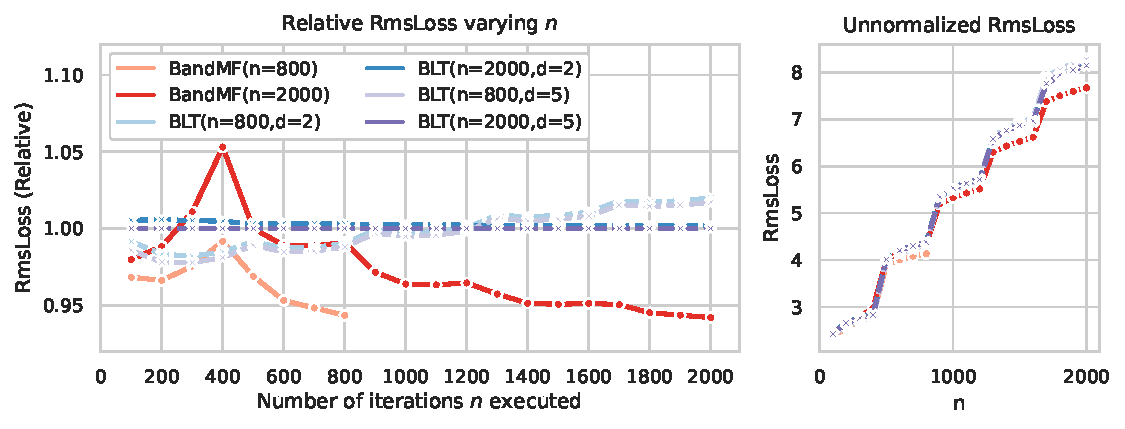
\includegraphics[width=\linewidth]{images/rmse_vary_n.pdf}
    \caption{Comparison of \bandmf and \blts optimized for $\nd=800$ and $\nd=2000$, and evaluated for $\nd$ up to the optimization target (for $\bandmf$) and over $[0, 2000]$ for the \blts. All mechanisms were optimized for min-separation (bands) $\minsep=400$. \blts with $\nbuf=2$ and $\nbuf=5$ perform almost equivalently; $\nbuf=1$ (not shown),is not sufficient with relative \rmsloss $> 1.07$.}
    \label{fig:rmse_vary_n}
\end{figure}

\begin{figure}[htb]
    \centering
    % FROM: https://colab.corp.google.com/drive/1_BRrt0jUniaOixKwasKDr7jiSToRwJLj#scrollTo=cYshzSOPA4wL&uniqifier=1
    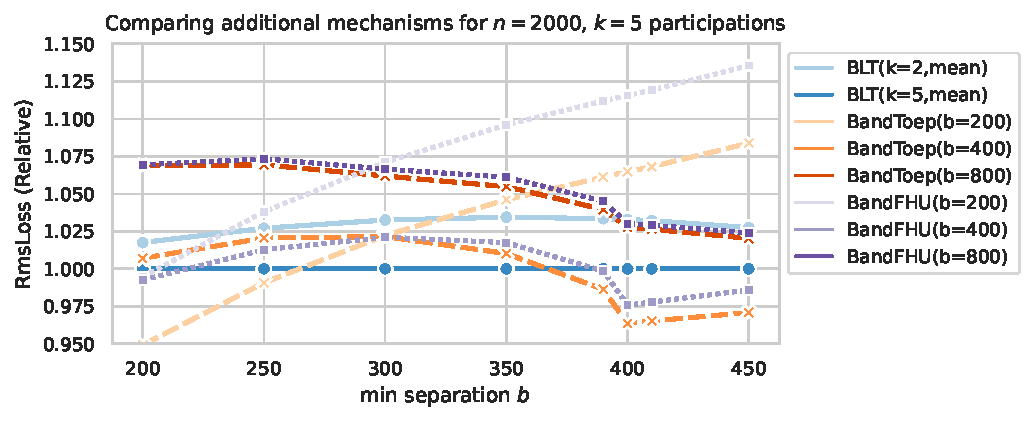
\includegraphics[width=\linewidth]{images/rmsloss_other_mechs.pdf}
    \caption{Comparison of mechanisms for $\nd=2000$ and $\maxpart=5$ participations, optimized for min-separation $\minsep = 400$ and compared for different actual values of min-separation. The setting is comparable to that of \cref{fig:rmse}, so only relative lines are given. 
    }
    \label{fig:other_mechs}
\end{figure}



\paragraph{Comparing \blt to \bandtoep and \bandfhu} Finally, we compare BLT-DP-FTRL to several other more recent mechanisms:
\begin{itemize}
    \item \bandtoep~\citep{mckenna2024scaling}, which optimizes banded Toeplitz matrices $\bfC$ for \bparticipation under \rmsloss. The primary advantage of this mechanism compared to \bandmf is that \bandtoep matrices can be optimized for much larger $\nd$. However, the runtime is the same as \bandmf, and the optimization is still slower than the optimization of \blts.
    \item \bandfhu~\citep{kalinin2024banded}, which uses prefixes of the optimal-for-single-participation \maxloss coefficients of \citet{fichtenberger2022constant} to form banded Toeplitz matrices. These will likely be worse than \bandtoep (which is specifically optimized for multiple participations), but require no mechanism optimization.
\end{itemize}
\cref{fig:other_mechs} shows that \blts are comparable or better to both of these approaches.}